\documentclass{beamer}
\usepackage[italian]{babel}
\usepackage{algorithm}
\usepackage{algpseudocode}
\usepackage{float}

\DeclareMathOperator{\lcm}{lcm}

\title{Presentazione PHPC}
\author{Pierluigi Supino \and Rodolfo Diana \and Salvatore Di Gennaro}

\usetheme{default}
\begin{document}
\begin{frame}
    \titlepage
\end{frame}

\begin{frame}{Implementazione}
    In ambiente multi-nodo e multi-GPU, il prodotto tra matrici viene scomposto in due sottoproblemi:
    \begin{enumerate}
        \item gestione a livello globale tra i processi, ovvero come suddividere le matrici e quali comunicazioni eseguire;
        \item gestione a livello locale all'interno di ciascun nodo, ovvero come eseguire il prodotto sfruttando le GPU a disposizione.
    \end{enumerate}
\end{frame}

\begin{frame}{Implementazione}{Processi}
    \begin{itemize}
        \item Scalable Universal Matrix Multiplication Algorithm (SUMMA)
        \item Algoritmo efficiente e scalabile per ogni numero di processi
    \end{itemize}
\end{frame}

\begin{frame}{Implementazione}{Processi}
    \begin{itemize}
        \item Si dispongono i processi in una griglia $r \times c$
        \item Si dividono le matrici $\mathbf{A}$ e $\mathbf{B}$ in $r \times \lcm(r,c)$ e $\lcm(r,c) \times c$ blocchi rispettivamente
        \item Si distribuiscono ciclicamente i blocchi delle matrici ai processi
    \end{itemize}
    \begin{figure}
        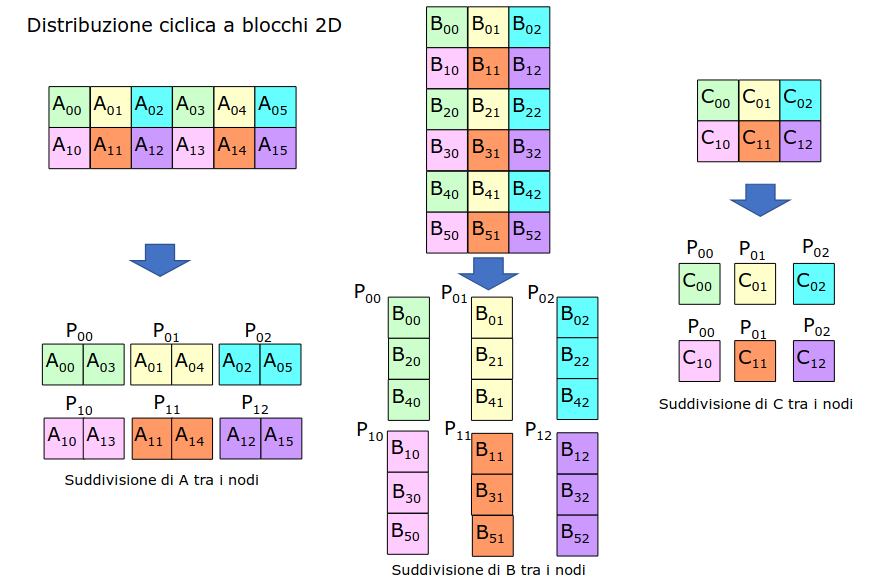
\includegraphics[width=0.5\linewidth]{imgs/summa.png}
        \caption{Distribuzione SUMMA}
    \end{figure}
\end{frame}

\begin{frame}{Implementazione}{Processi}
    \begin{itemize}
        \item Per $\lcm(r,c)$ volte:
              \begin{enumerate}
                  \item Un processo invia il suo blocco di $\mathbf{A}$ alla propria riga
                  \item Un processo invia il suo blocco di $\mathbf{B}$ alla propria colonna
                  \item Viene sommato il prodotto parziale dei blocchi ricevuti
              \end{enumerate}
    \end{itemize}
    \begin{figure}
        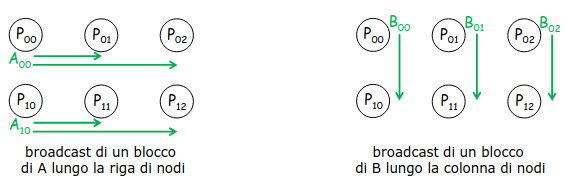
\includegraphics[width=0.5\linewidth]{imgs/broadcast_1.jpg}
        \caption{Esempio di broadcast}
    \end{figure}
\end{frame}

\begin{frame}{Implementazione}{Processi}
    \begin{algorithm}[H]
        \caption{SUMMA for process $P_{i,j}$}
        \begin{algorithmic}[1]
            \State $\mathbf{C}^{i,j} \gets 0$
            \State $l \gets \lcm(r,c)$
            \For{$k \gets 0$ \textbf{to} $l - 1$}
            \State $s \gets \bmod(k, r)$
            \State $t \gets \bmod(k, c)$
            \State process $P_{it}$ broadcasts $\mathbf{A}^{i,k}$ to its row
            \State process $P_{sj}$ broadcasts $\mathbf{B}^{k,j}$ to its column
            \State $\mathbf{C}^{i,j} \gets \mathbf{C}^{i,j} + \mathbf{A}^{i,k}\mathbf{B}^{k,j}$
            \EndFor
        \end{algorithmic}
    \end{algorithm}
\end{frame}

\begin{frame}{Implementazione}{Processi}
    Semplificazioni e assunzioni effettuate:
    \begin{itemize}
        \item solo matrici quadrate $n \times n$, con $n$ multiplo di $\lcm(r,c)$
        \item matrici di input di ogni processo come array contigui \textit{row-major} contenenti già i dati necessari
        \item gestione degli errori quasi assente per evitare overhead
    \end{itemize}
\end{frame}

\begin{frame}{Implementazione}{GPU}
    \begin{itemize}
        \item Più GPU per processo: come suddividere il lavoro?
              \begin{itemize}
                  \item Vogliamo eseguire le operazioni in parallelo
                        \begin{enumerate}
                            \item Evitare conflitti di memoria da serializzare
                            \item Nessuna funzione bloccante per l'host
                        \end{enumerate}
              \end{itemize}
        \item Possibili soluzioni:
              \begin{itemize}
                  \item Pattern fork-join con ogni thread che gestisce una GPU
                  \item \alert{Utilizzo dei metodi async e degli stream di CUDA}
              \end{itemize}
    \end{itemize}
\end{frame}


\begin{frame}{Implementazione}{GPU}
    \begin{itemize}
        \item CUDA stream: code di operazioni da gestire in sequenza
              \begin{itemize}
                  \item Operazioni in stream diversi potrebbero essere eseguite in concorrenza oppure alternate
                  \item Se non viene specificato uno stream viene usato lo stream 0 (bloccante)
              \end{itemize}
              % \item Host crea stream per ogni device e specifica operazioni asincrone da eseguire
        \item I trasferimenti sono davvero asincroni solo se la memoria indirizzata è \textit{page-locked}
              \begin{itemize}
                  \item cudaMallocHost
                  \item cudaHostRegister/cudaHostUnregister
              \end{itemize}
    \end{itemize}
\end{frame}

\begin{frame}{Implementazione}{GPU - cuBLAS}
    \begin{itemize}
        \item Problema del prodotto matriciale già ampiamente discusso
        \item Numerose librerie disponibili: \alert{cuBLAS}
              \begin{itemize}
                  \item implementazione ottimizzata per GPU NVIDIA delle specifiche BLAS
                        \begin{itemize}
                            \item Per compatibilità con Fortran si aspetta ordine column-major
                            \item Basta calcolare $\mathbf{C}^T=(\mathbf{B}\mathbf{A})^T$
                        \end{itemize}
                  \item \alert{cuBLASXt}: estensione per ambienti multi-GPU
              \end{itemize}
    \end{itemize}
\end{frame}

\begin{frame}{Implementazione}{Kernel 1}
    \begin{itemize}
        \item Per implementare la moltiplicazione tra matrici in CUDA possiamo:
            \begin{itemize}
                \item Mappare i thread della griglia agli elementi della matrice di output in modo che ognugno sia responsabile del calcolo del singolo elemento.
                \item Gli indici dell'elemento che ogni thread dovrà calcolare saranno:
                    \begin{itemize}
                        \item \textit{row = blockIdx.y × blockDim.y + threadIdx.y}
                        \item \textit{col = blockIdx.x × blockDim.x + threadIdx.x}
                    \end{itemize}
            \end{itemize}
    \end{itemize}
\end{frame}

\begin{frame}{Implementazione}{Kernel 1}
    \begin{algorithm}[H]
    \caption{Matrix Multiplication Kernel 1}
    \begin{algorithmic}[1]
    \State $\texttt{row} \gets \texttt{blockIdx.y} \cdot \texttt{blockDim.y} + \texttt{threadIdx.y}$
    \State $\texttt{col} \gets \texttt{blockIdx.x} \cdot \texttt{blockDim.x} + \texttt{threadIdx.x}$
    \If{$\texttt{row} < \texttt{Width}$ \textbf{and} $\texttt{col} < \texttt{Width}$}
        \State $\texttt{Pval} \gets 0$
        \For{$k \gets 0$ \textbf{to} $\texttt{Width} - 1$}
            \State $\texttt{Pval} \gets \texttt{Pval} + M[\texttt{row} \cdot \texttt{Width} + k] \cdot N[k \cdot \texttt{Width} + \texttt{col}]$
        \EndFor
        \State $P[\texttt{row} \cdot \texttt{Width} + \texttt{col}] \gets \texttt{Pval}$
    \EndIf
    \end{algorithmic}
    \end{algorithm}
\end{frame}

\begin{frame}{Implementazione}{Kernel 1}
    \begin{figure}[H]
        \centering
        \begin{minipage}{0.48\textwidth}
            \centering
            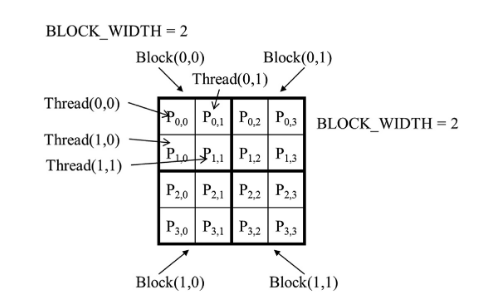
\includegraphics[width=\linewidth]{imgs/matrix_division.png}
            \caption{Figura 1: Divisione degli elementi in una griglia 2x2 con blocchi 2x2}
        \end{minipage}
        \hfill
        \begin{minipage}{0.48\textwidth}
            \centering
            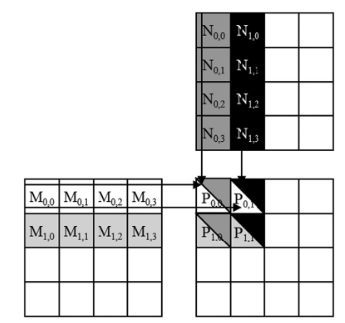
\includegraphics[width=\linewidth]{imgs/execution1.png}
            \caption{Figura 2: Esempio di calcolo}
        \end{minipage}
    \end{figure}
\end{frame}

\begin{frame}{Implementazione}{Kernel 1}
    \begin{itemize}
        \item Ampi margini di miglioramento rispetto alla memoria
        \begin{itemize}
            \item La memoria globale è grande ma lenta
             \item La memoria condivisa è piccola ma veloce
        \end{itemize}
    \end{itemize}
    \begin{figure}[H]
        \centering
        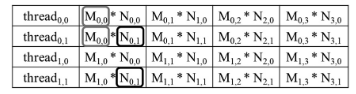
\includegraphics[width=0.7\textwidth]{imgs/memory_access.png}
    \end{figure}
    \begin{itemize}
        \item Idea: Partizionare i dati in sottoinsiemi chiamati tiles, in modo tale che ognuna di essa entri nella memoria condivisa. Tutti i thread collaboreranno al caricamento delle tiles in memoria condivisa prima della computazione. Stiamo riducendo gli accessi alla memoria globale di un fattore $\frac{1}{width}$
    \end{itemize}
\end{frame}

\begin{frame}{Implementazione}{Kernel 2}
    \begin{figure}[H]
        \centering
        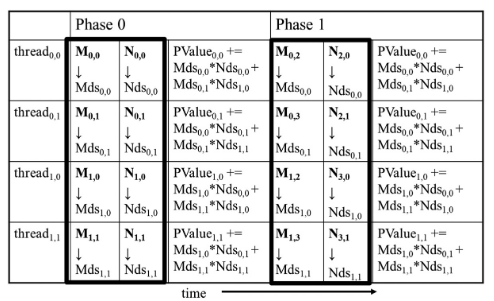
\includegraphics[width=0.7\textwidth]{imgs/memory_access1.png}
        \caption{Figura 3: Accessi alla memoria nuovo approccio}
    \end{figure}
\end{frame}

\begin{frame}{Implementazione}{Kernel 2}
    \begin{algorithm}[H]
    \caption{Tiled Matrix Multiplication Kernel 2}
    \begin{algorithmic}[1]
    \State \texttt{Pval} $\gets$ 0
    \For{$ph \gets 0$ \textbf{to} $\texttt{Width} / \texttt{TILE\_WIDTH} - 1$}
        \State $M_{ds}[ty][tx] \gets M[Row \cdot Width + ph \cdot TILE\_WIDTH + tx]$
        \State $N_{ds}[ty][tx] \gets N[(ph \cdot TILE\_WIDTH + ty) \cdot Width + Col]$
        \State \texttt{syncthreads()}
        \For{$k \gets 0$ \textbf{to} \texttt{TILE\_WIDTH} - 1}
            \State \texttt{Pval} $\gets$ \texttt{Pval} $+$ $M_{ds}[ty][k] \cdot N_{ds}[k][tx]$
        \EndFor
        \State \texttt{syncthreads()}
    \EndFor
    \State $P[Row \cdot Width + Col] \gets$ \texttt{Pval}
    \end{algorithmic}
    \end{algorithm}
\end{frame}

\begin{frame}{Implementazione}{Kernel 2}
\begin{algorithm}[H]
\scriptsize
\caption{Tiled Matrix Multiplication Kernel 2 con padding}
\begin{algorithmic}[1]
\State $Pval \gets 0$
\For{$ph \gets 0$ \textbf{to} $\lceil W/T \rceil -1$}
  \State $M_{ds}[ty][tx] \gets (Row<W~\&\&~ph\cdot T+tx<W)~?~M[Row\cdot W + ph\cdot T + tx]~:~0$
  \State $N_{ds}[ty][tx] \gets (ph\cdot T+ty<W~\&\&~Col<W)~?~N[(ph\cdot T+ty)\cdot W + Col]~:~0$
  \State \texttt{syncthreads()}
  \For{$k \gets 0$ \textbf{to} $T-1$}
    \State $Pval \mathrel{+}= M_{ds}[ty][k] \cdot N_{ds}[k][tx]$
  \EndFor
  \State \texttt{syncthreads()}
\EndFor
\If{$Row < W~\&\&~Col < W$}
  \State $P[Row\cdot W + Col] \gets Pval$
\EndIf
\end{algorithmic}
\end{algorithm}
\end{frame}

\begin{frame}{Implementazione}{Kernel 3}
    \begin{itemize}
        \item TODO
    \end{itemize}
\end{frame}

\end{document}